\documentclass{beamer}


\usepackage[french,english]{babel}

\usepackage[T1]{fontenc}

\usepackage[utf8]{inputenc}
\usepackage[linesnumbered,ruled,vlined]{algorithm2e}

\usetheme{Warsaw}
\definecolor{rouge}{HTML}{DD0000}
\title{Présentation stage}

\author{Clément Legrand}

\begin{document}


\begin{frame}[plain]
\titlepage
\end{frame}

\section{Présentation du problème}

\subsection{Capacitated Vehicle Routing Problem (CVRP)}
\footnotesize
\begin{frame}{Capacitated Vehicle Routing Problem}
\begin{block}{Notations}
Instance $I$ : $n$ clients et 1 dépôt

Solution $Sol$ : $k$ tournées

La demande $d_i$ du client $i$, une capacité $C$
\end{block}
\begin{alertblock}{Règles}
\begin{itemize}
\item $\forall i > 0 \in I$, $\exists! R_j \in Sol, i \in R_j$;
\item Chaque tournée doit partir et s'arrêter au dépôt;
\item $ \forall R_j \in Sol, \sum_{i \in R_j} d_i \leq C$.
\end{itemize}
\end{alertblock}
\begin{exampleblock}{Objectif}
Déterminer $Sol$ tel que:

\centering
$ Sol = argmin_{Sol} \sum_{R_j \in Sol} \sum_{i = 0}^{|R_j|-1} dist(R_j[i],R_j[i+1]) = argmin_{Sol}cost(Sol)$
\end{exampleblock}
\end{frame}

\begin{frame}{Exemple}
Instance A-n37-k06:
 \begin{columns}[t]
  \begin{column}{5cm}
  	\centering
	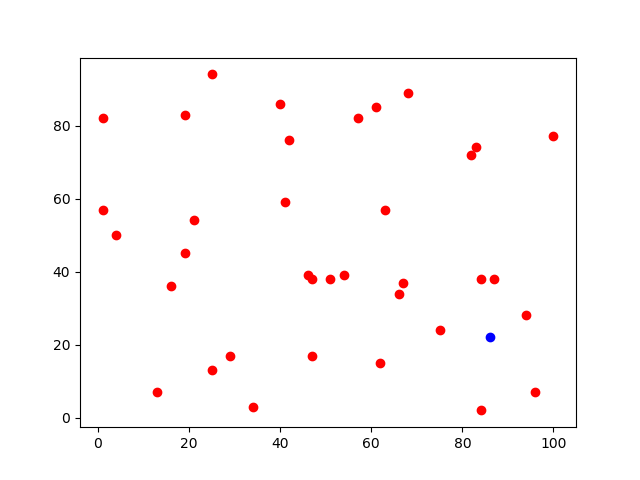
\includegraphics[scale=0.32]{instanceA3706.png}
	
	Représentation instance 
  \end{column}
  
  \begin{column}{5cm}
  	\centering
	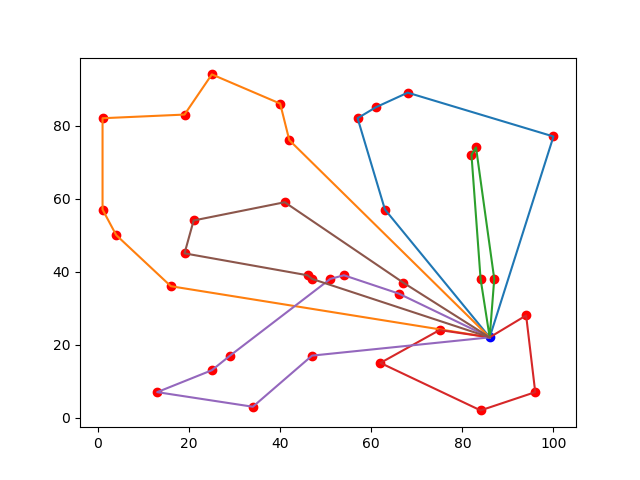
\includegraphics[scale=0.32]{bestA3706.png}
 
 	Meilleure solution connue
  \end{column}
 \end{columns}

\end{frame}

\subsection{Motivation}

\begin{frame}
\begin{block}{Objectif}
Intégrer de la connaissance lors du calcul d'une solution
\end{block}

\begin{exampleblock}{Idée}
Prédire les arêtes optimales en apprenant à partir de solutions initiales de bonne qualité
\end{exampleblock}

\begin{alertblock}{Problèmes}
\begin{itemize}
\item Comment construire une solution initiale de bonne qualité ?
\item Quelle heuristique utiliser ?
\item Comment extraire la connaissance ?
\item Comment intégrer la connaissance dans l'heuristique ?
\end{itemize}
\end{alertblock}
\end{frame}

\section{Construction solution initiale}

\subsection{Algorithme CW}


\begin{frame}{Algorithme Clarke \& Wright (CW)}

CW\footnote{IK. Altinel and T. Öncan, A new enhancement of the Clarke and Wright savings heuristic for the capacitated vehicle routing problem (2005)}$\rightarrow$ Algorithme glouton. 

\begin{exampleblock}{Définition saving}
Calcul du saving de $i$ et $j$ avec:
\begin{center}
$s(i,j) = c_{i0} + c_{0j} - \lambda c_{ij} + \mu \vert c_{i0} - c_{0j} \vert + \nu \frac{d_i + d_j}{\overline{d}}$
\end{center}
$(\lambda,\mu,\nu)$ sont des paramètres à déterminer
\end{exampleblock}

\begin{block}{Fonctionnement}
Tant que $max_{(i,j)}s(i,j) > 0$:
\begin{itemize}
\item $(i,j) \leftarrow argmax_{(i,j)}s(i,j)$;
\item Les tournées qui contiennent $i$ et $j$ sont fusionnées (si possible);
\item $s(i,j) \leftarrow  0$.
\end{itemize} 

\end{block}
\end{frame}

\subsection{Exemple d'exécution}
\begin{frame}{Exécution pour $(\lambda,\mu,\nu) = (1,1,1)$}

 \begin{columns}[t]
  \begin{column}{4cm}
  	\centering
	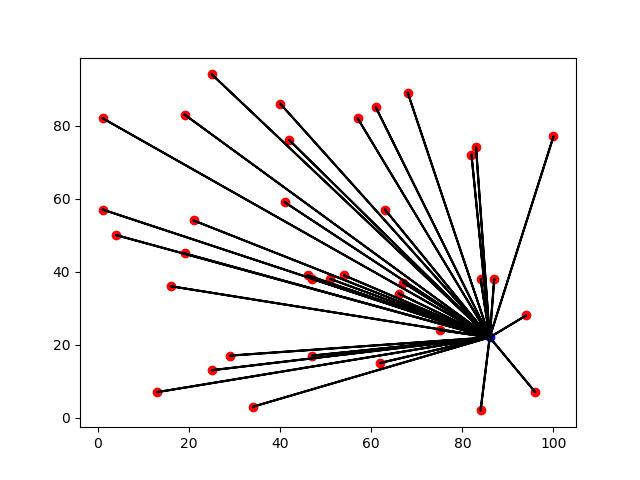
\includegraphics[scale=0.25]{CWinit.png}
	
	Initialisation
  \end{column}
  
  \begin{column}{4cm}
  	\centering
	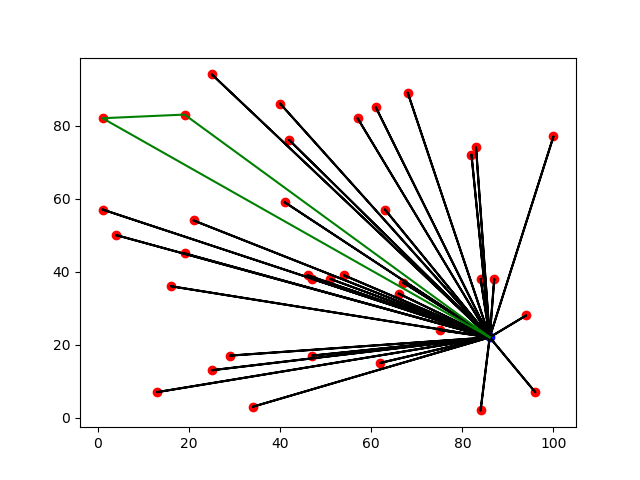
\includegraphics[scale=0.25]{CW1.png}
 
 	1$^{ere}$ fusion
  \end{column}

 
  \begin{column}{4cm}
  	\centering
	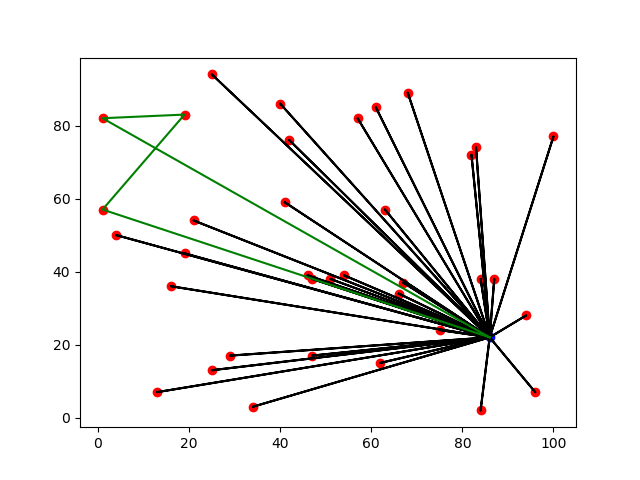
\includegraphics[scale=0.25]{CW2.png}
 	2$^{eme}$ fusion

  \end{column}
 \end{columns}
 
 \centering
 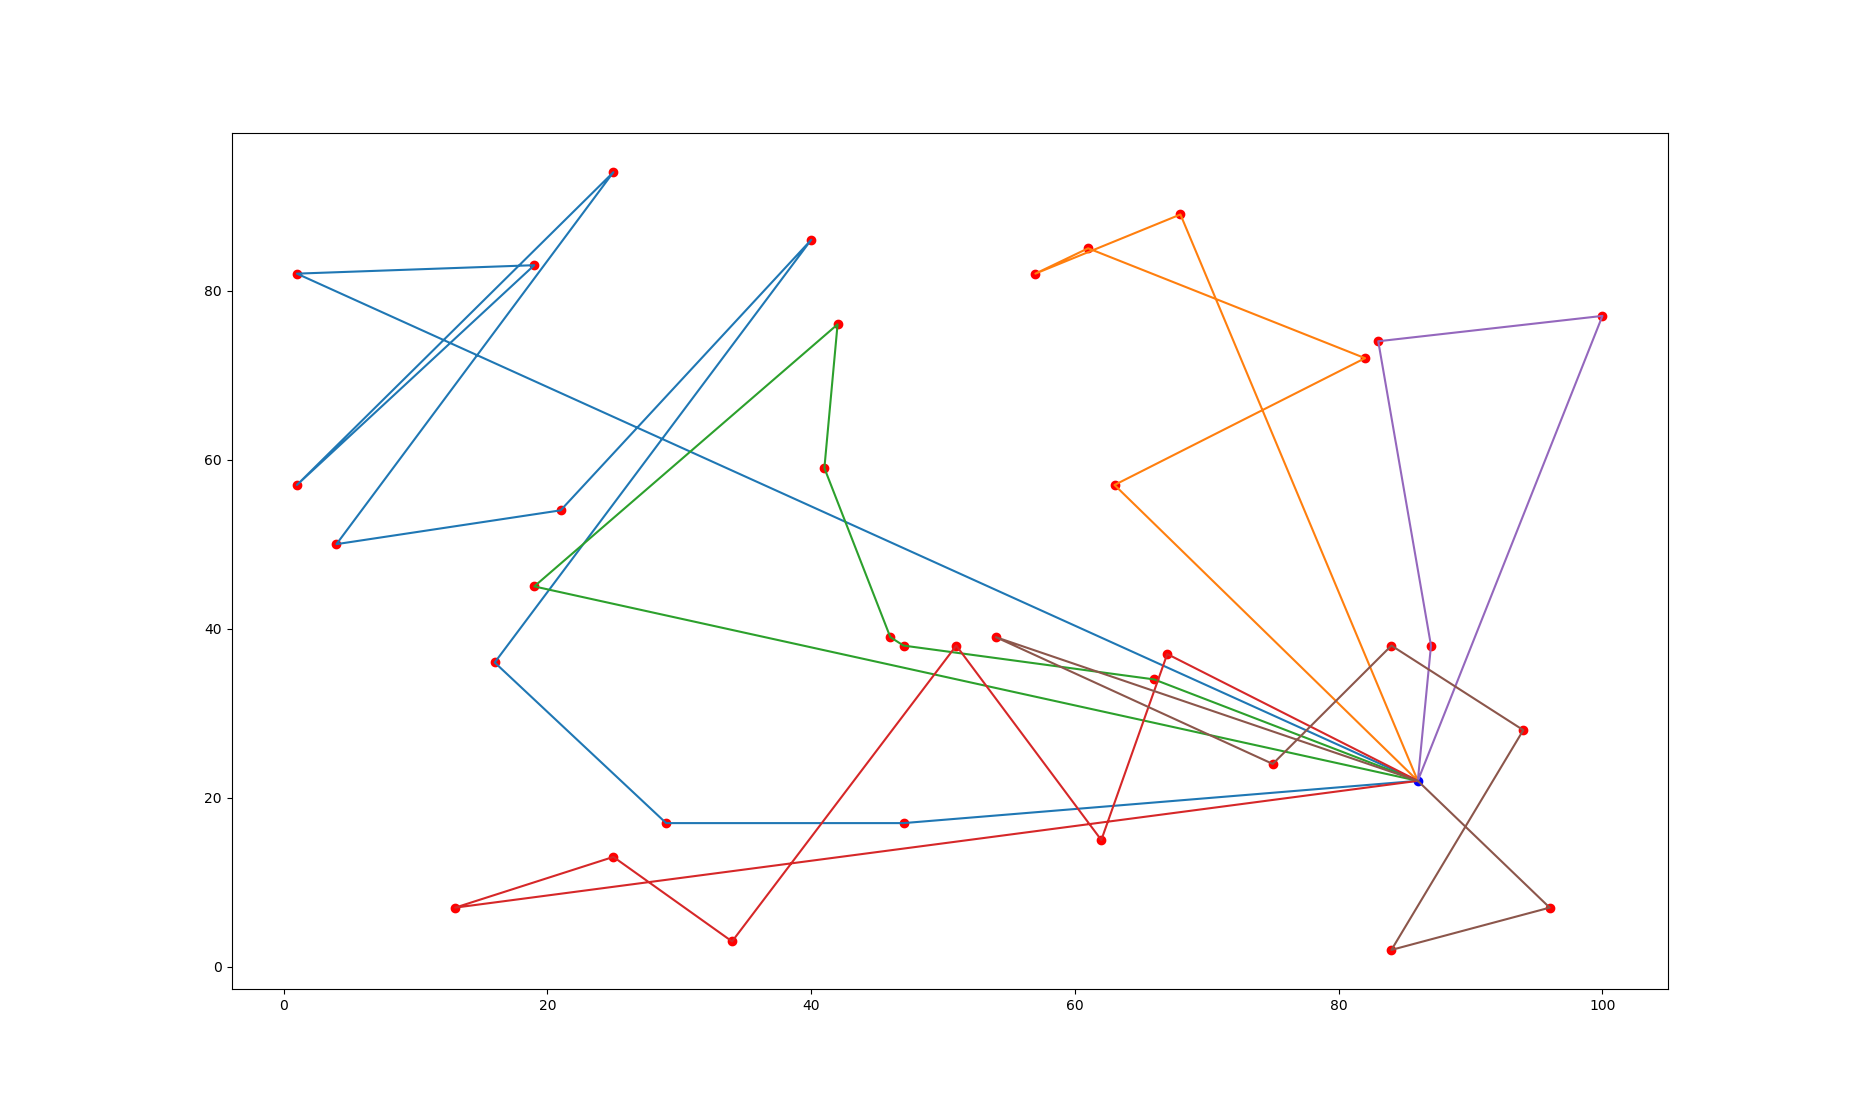
\includegraphics[scale=0.13]{resCW101010.png}
\end{frame}

\subsection{Problème de $(\lambda,\mu,\nu)$}

\begin{frame}{Choix de $(\lambda,\mu,\nu)$ ?}

 \begin{columns}[t]
  \begin{column}{4cm}
  	\centering
	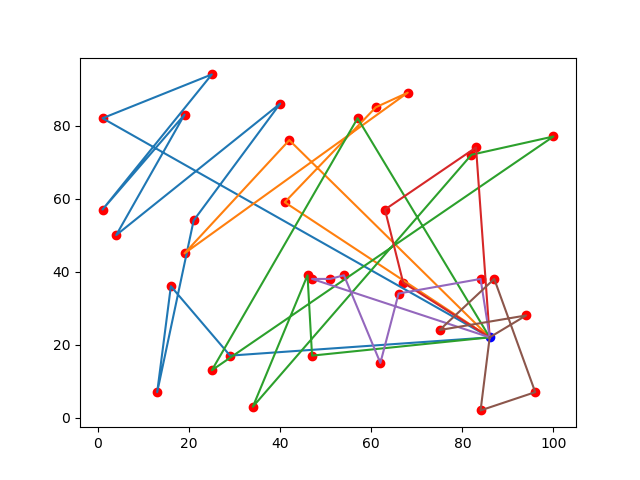
\includegraphics[scale=0.27]{resCW111.png}
	
	$(0.1,0.1,0.1), cost = 1569$
  \end{column}
  
  \begin{column}{4cm}
  	\centering
	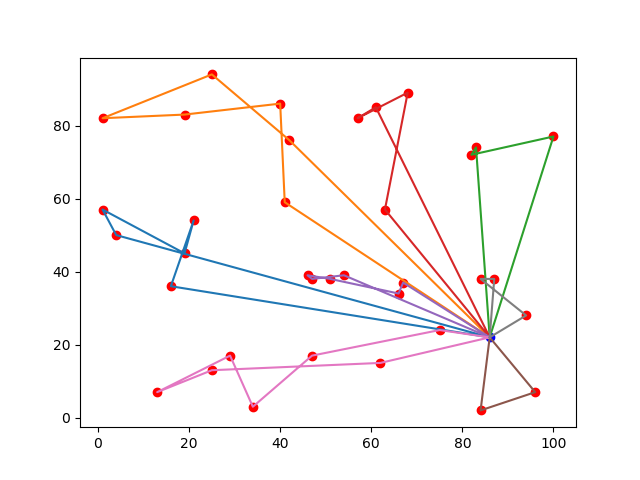
\includegraphics[scale=0.27]{resCW190105.png}
 
 	$(1.9,0.1,1.5), cost = 1106$
  \end{column}

 
  \begin{column}{4cm}
  	\centering
	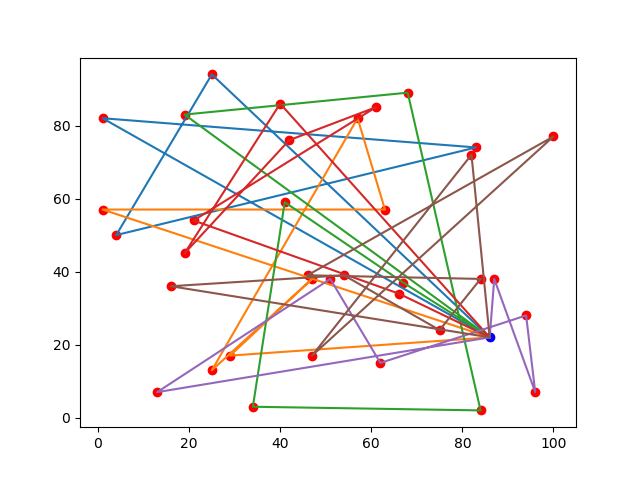
\includegraphics[scale=0.27]{resCW001015.png}
 	$(0.0,1.0,1.5), cost = 2191$

  \end{column}
 \end{columns}
 
\begin{alertblock}{Bilan}
Difficile de prévoir l'influence des paramètres
\end{alertblock}

\end{frame}

\section{Choix de l'heuristique}

\subsection{Heuristique A \& S}

\begin{frame}{Heuristique Arnold \& Sörensen} 

\begin{algorithm}[H]
\DontPrintSemicolon % Some LaTeX compilers require you to use \dontprintsemicolon instead

$Sol \gets CW(\lambda,\mu,\nu)$\;
$NewSol \gets Sol$\;
\While {Pas d'améliorations depuis 3 min} {
	Calcul de la pire arête\;
	$NewSol \gets EjectionChain_{BI-O}$\;
	$NewSol \gets LinKernighan_{BI-O}$\;
	$NewSol \gets CrossExchange_{BI-O}$\;
	$NewSol \gets LinKernighan_{BI-O}$\;
	\If {$cost(NewSol) < cost(Sol)$} {
		$Sol \gets NewSol$\;
	}
}
\Return{$Sol$}\;

\end{algorithm}

\end{frame}

\subsection{Détail des opérations}

\begin{frame}{Pire arête}
\begin{exampleblock}{Pire arête}
La pire arête du graphe est l'arête $(i,j)$ qui maximise la fonction:
\begin{center}
$b(i,j) = \frac{[\gamma_w w(i,j) + \gamma_c c(i,j)] [\frac{d(i,j)}{max_{k,l}d(k,l)}] ^ {\frac{\gamma_d}{2}}}{1+p(i,j)}$
\end{center}
\end{exampleblock}

\begin{figure}
\centering
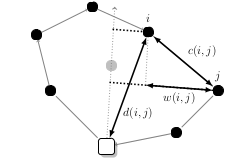
\includegraphics[scale=0.6]{metrics.png}
\end{figure}

\end{frame}

\begin{frame}{Opérateurs locaux}
\begin{block}{Ejection-chain}
Déplacer $l$ clients sur des tournées. 
\end{block}
\begin{block}{Cross-exchange}
Échanger deux séquences de clients entre deux tournées. 
\end{block}
\begin{figure}
	\centering
	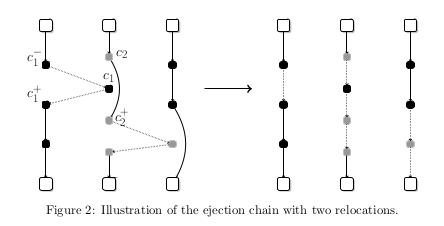
\includegraphics[scale=0.3]{ejection_chain.png}
	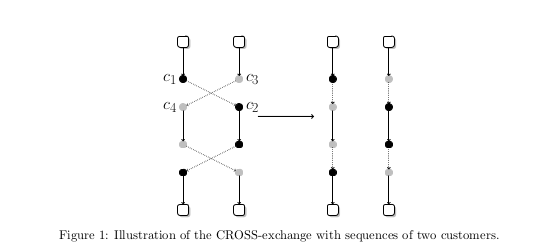
\includegraphics[scale=0.3]{cross_exchange.png}
\end{figure}

\end{frame}

\begin{frame}{Opérateurs locaux}
\begin{block}{Lin-Kernighan}
\begin{itemize}
\item Utilisé en général pour TSP;
\item Optimisation intra-tournée (chaque tournée est améliorée indépendamment des autres).
\end{itemize}
\end{block}
\begin{figure}
	\centering
	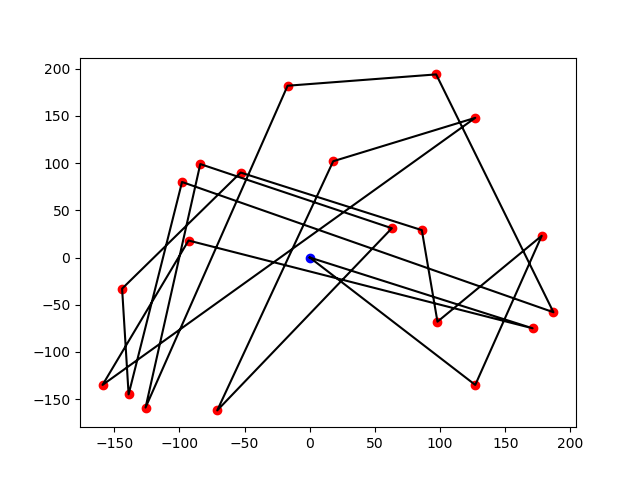
\includegraphics[scale=0.3]{test4_20_init.png}
	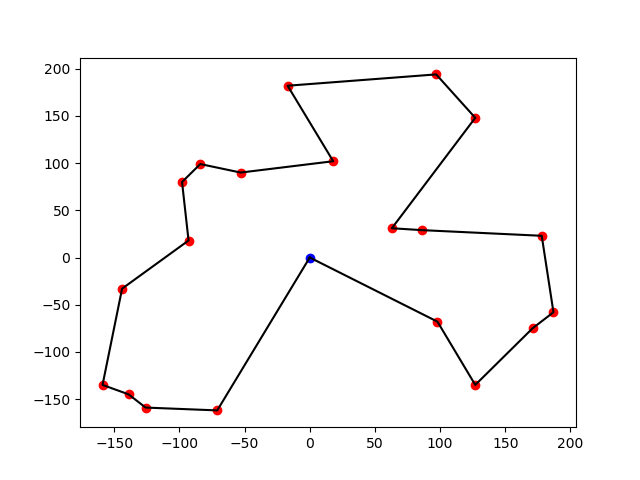
\includegraphics[scale=0.3]{test4_20_LKopt.png}
\end{figure} 
\end{frame}

\subsection{Heuristique utilisée}

\begin{frame}{Heuristique utilisée ($H_c$)}

\begin{algorithm}[H]
\DontPrintSemicolon % Some LaTeX compilers require you to use \dontprintsemicolon instead

$Sol \gets CW(\lambda,\mu,\nu)$\;
$NewSol \gets Sol$\;
\While {La dernière amélioration date de moins de \textcolor{rouge}{$n/3$ min}} {
	Calcul de la pire arête\;
	$NewSol \gets EjectionChain_{\textcolor{rouge}{FI-RD}}$\;
	$NewSol \gets LinKernighan_{BI-O}$\;
	$NewSol \gets CrossExchange_{\textcolor{rouge}{FI-RD}}$\;
	$NewSol \gets LinKernighan_{BI-O}$\;
	\If {$cost(NewSol) < cost(Sol)$} {
		$Sol \gets NewSol$\;
	}
	\textcolor{rouge}{
	\If {Pas d'améliorations depuis $n/2$ itérations}{
		$NewSol \gets Sol$\;
	}
	}
}
\Return{$Sol$}\;

\end{algorithm}
\end{frame}

\begin{frame}{Validation}

\begin{tabular}{|c|c|c|c|c|c|c|c|c|c|}
   \hline
    & \multicolumn{3}{c|}{A-n37-k06} & \multicolumn{3}{c|}{A-n65-k09} & \multicolumn{3}{c|}{P-n101-k04} \\
   \hline
   Ajout & Best & Mean & Time & Best & Mean & Time & Best & Mean & Time \\
   \hline
   Rien &  950 & 957 & 195 & 1197 & 1215 & 395 & 722 & 736 & 783  \\   
   \hline
   Divers & 950 & 969 & 200 & 1200 & 1230 & 350 & 698 & 706 & 1500  \\
   \hline
\end{tabular}

\begin{block}{Conclusion}
Diversification plus intéressante pour des grandes instances
\end{block}



\end{frame}


\section{Extraction des connaissances}

\subsection{Contribution}

\begin{frame}{Exemples}
 \begin{columns}[t]
  \begin{column}{4cm}
  	\centering
	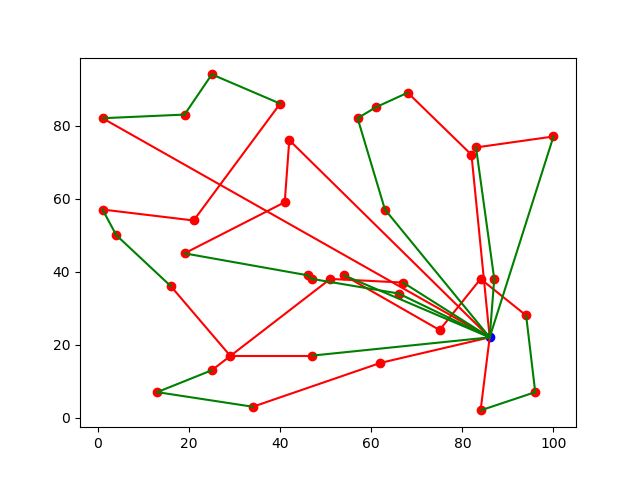
\includegraphics[scale=0.25]{edges101010.png}
	
  \end{column}
  
    \begin{column}{4cm}
  	\centering
	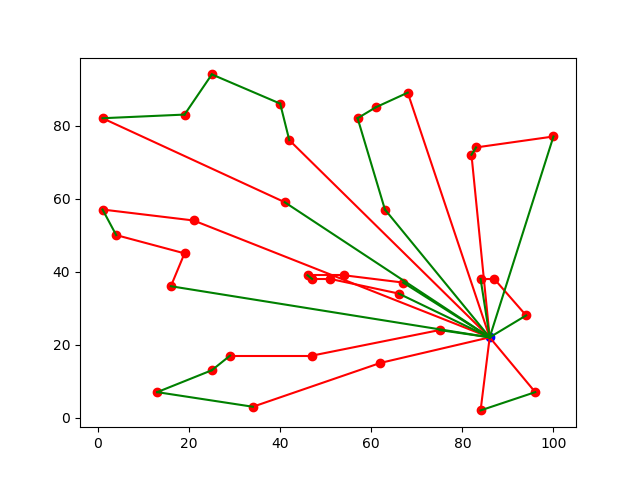
\includegraphics[scale=0.25]{edges190115.png}


  \end{column}
  
  \begin{column}{4cm}
  	\centering
	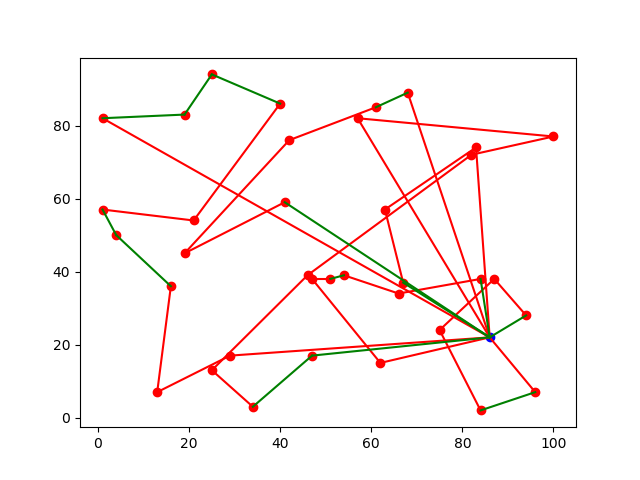
\includegraphics[scale=0.25]{edges010101.png}

  \end{column}

 

 \end{columns}
 
 \centering
 $\downarrow$
 
 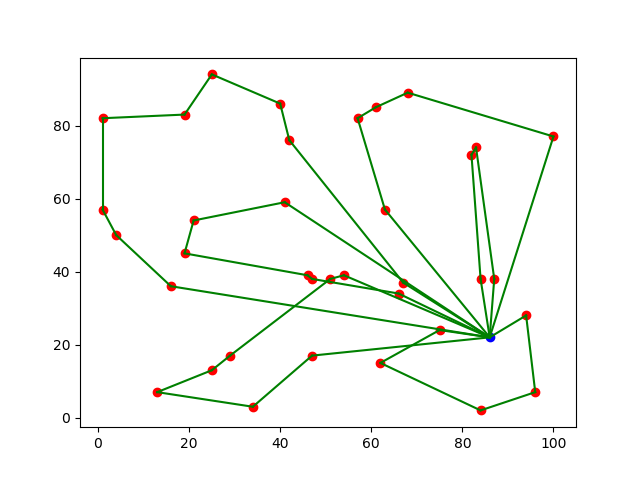
\includegraphics[scale=0.25]{edgesSol.png}
\end{frame}

\begin{frame}{Protocole}
\begin{alertblock}{Questions}
\begin{itemize}
\item Combien de solutions dans l'échantillon ?
\item Combien de solutions pour apprendre ?
\item Comment choisir les arêtes à conserver ?
\end{itemize}
\end{alertblock}
\end{frame}

\begin{frame}{Protocole}

\begin{block}{Combien de solutions dans l'échantillon ?}
\begin{itemize}
\item Considérer tous les $(\lambda,\mu,\nu)$;
\item Tirer $N$ $(\lambda,\mu,\nu)$ aléatoirement;
\end{itemize}
\end{block}

\begin{block}{Quelles solutions pour apprendre ?}
\begin{itemize}
\item Tout l'échantillon (Tout);
\item $x\%$ des meilleures solutions : quantité privilégiée (Quan$_{x}$);
\item Solutions avec coût inférieur à $c_{min} + (c_{max}-c_{min})\frac{x}{100}$ : qualité privilégiée (Qual$_{x}$);
\end{itemize}
\end{block}

\begin{block}{Comment choisir les arêtes à conserver ?}
Pour chaque arête (i,j), on incrémente la valeur de MAT[i][j];
\begin{itemize}
\item Conserver $(i,j) \Leftrightarrow MAT[i][j] > seuil$ (Seuil);
\item Conserver les $rg$ premières arêtes dans la matrice (Rang).
\end{itemize}
\end{block}


\end{frame}

\subsection{Validation}
\begin{frame}{Résultats}

\begin{table}[H]

\begin{tabular}{|@{}c@{}|@{}c@{}|@{}c@{}|@{}c@{}|@{}c@{}||@{}c@{}|@{}c@{}|@{}c@{}|@{}c@{}||@{}c@{}|@{}c@{}|@{}c@{}|@{}c@{}|}

\hline
 & \multicolumn{4}{c|}{Quan$_{10}$} & \multicolumn{4}{c|}{Qual$_{10}$} & \multicolumn{4}{c|}{Tout} \\
 \hline
 & Seuil & Arêtes & Corr & Prop & Seuil & Arêtes & Corr & Prop & Seuil & Arêtes & Corr & Prop \\
 \hline
 50 & 3 & 34 & 21 & 0.5 & L$_{lb}$/2 & 33 & 21 & 0.50 & 25 & 23 & 15 & 0.35 \\
 \cline{2-13} 
    & 4 & 23 & 14 & 0.33 & 3L$_{lb}$/4 & 17 & 12 & 0.28 & 38 & 10 & 7 & 0.16 \\
  \hline
   100 & 5 & 30 & 21 & 0.5 & L$_{lb}$/2 & 31 & 23 & 0.55 & 50 & 24 & 17 & 0.40 \\
 \cline{2-13} 
    & 8 & 16 & 15 & 0.36 & 3L$_{lb}$/4 & 17 & 14 & 0.33 & 75 & 6 & 6 & 0.14 \\
  \hline
   500 & 25 & 32 & 24 & 0.57 & L$_{lb}$/2 & 31 & 22 & 0.52 & 250 & 22 & 15 & 0.36 \\
 \cline{2-13} 
    & 38 & 15 & 14 & 0.33 & 3L$_{lb}$/4 & 20 & 16 & 0.38 & 375 & 7 & 7 & 0.18 \\
  \hline
   8000 & 400 & 33 & 24 & 0.57 & L$_{lb}$/2 & 30 & 23 & 0.55 & 4000 & 25 & 16 & 0.38 \\
 \cline{2-13} 
    & 600 & 15 & 14 & 0.33 & 3L$_{lb}$/4 & 18 & 16 & 0.38 & 6000 & 9 & 6 & 0.14 \\
  \hline

\end{tabular}


\end{table}
\end{frame}

\begin{frame}{Résultats}
\begin{table}[H]

\begin{tabular}{|@{}c@{}|@{}c@{}|@{}c@{}|@{}c@{}||@{}c@{}|@{}c@{}|@{}c@{}||@{}c@{}|@{}c@{}|@{}c@{}|}

\hline
 & \multicolumn{3}{c|}{Quan$_{10}$} & \multicolumn{3}{c|}{Qual$_{10}$} & \multicolumn{3}{c|}{Tout} \\
 \hline
 & Rang & Corr & Prop & Rang & Corr & Prop & Rang & Corr & Prop \\
 \hline
 50 & 10  & 6 & 0.14 & 10  & 6 & 0.14 & 10  & 7 & 0.16  \\
 \cline{2-10} 
    & 20 & 13 & 0.31 & 20  & 13 & 0.32 & 20  & 13 & 0.31  \\
 \cline{2-10} 
    & 18 & 12 & 0.28 & 18 & 13 & 0.3 & 18 & 12 & 0.28  \\
  \hline
   100 & 10  & 9 & 0.21 & 10  & 9 & 0.21 & 10  & 10 & 0.24  \\
 \cline{2-10} 
    & 20 & 16 & 0.38 & 20 & 16 & 0.38 & 20 & 15 & 0.36  \\
  \cline{2-10} 
    & 18 & 13 & 0.3 & 18 & 13 & 0.3 & 18 & 12 & 0.29  \\
  \hline
   500 & 10  & 9 & 0.21 & 10  & 10 & 0.24 & 10  & 9 & 0.21  \\
 \cline{2-10} 
    & 20 & 16 & 0.38 & 20 & 16 & 0.38 & 20 & 15 & 0.36  \\
  \cline{2-10} 
    & 18 & 13 & 0.3 & 18 & 13 & 0.3 & 18 & 12 & 0.28  \\
  \hline
   8000 & 10 & 8 & 0.19 & 10 & 9 & 0.21 & 10 & 7 & 0.17  \\
 \cline{2-10} 
    & 20 & 14 & 0.33 & 20 & 14 & 0.33 & 20 & 14 & 0.33  \\
  \cline{2-10} 
    & 18 & 12 & 0.29 & 18 & 12 & 0.29 & 18 & 12 & 0.29  \\
  \hline

\end{tabular}
\end{table}
\end{frame}


\begin{frame}{Résultats}

\begin{table}[H]

\begin{tabular}{|@{}c@{}|@{}c@{}|@{}c@{}|@{}c@{}|@{}c@{}||@{}c@{}|@{}c@{}|@{}c@{}|@{}c@{}||@{}c@{}|@{}c@{}|@{}c@{}|@{}c@{}|}

\hline
 & \multicolumn{4}{c|}{Quan$_{10}$} & \multicolumn{4}{c|}{Qual$_{10}$} & \multicolumn{4}{c|}{Tout} \\
 \hline
 & Seuil & Arêtes & Corr & Prop & Seuil & Arêtes & Corr & Prop & Seuil & Arêtes & Corr & Prop \\
 \hline
 50 & 3 & 34 & 21 & 0.5 & L$_{lb}$/2 & 33 & 21 & 0.50 & 25 & 23 & 15 & 0.35 \\
 \cline{2-13} 
    & 4 & 23 & 14 & 0.33 & 3L$_{lb}$/4 & 17 & 12 & 0.28 & 38 & 10 & 7 & 0.16 \\
  \hline
   100 & 5 & 30 & 21 & 0.5 & L$_{lb}$/2 & 31 & 23 & 0.55 & 50 & 24 & 17 & 0.40 \\
 \cline{2-13} 
    & 8 & 16 & 15 & 0.36 & 3L$_{lb}$/4 & 17 & 14 & 0.33 & 75 & 6 & 6 & 0.14 \\
  \hline
   500 & 25 & 32 & 24 & 0.57 & L$_{lb}$/2 & 31 & 22 & 0.52 & 250 & 22 & 15 & 0.36 \\
 \cline{2-13} 
    & 38 & 15 & 14 & 0.33 & 3L$_{lb}$/4 & 20 & 16 & 0.38 & 375 & 7 & 7 & 0.18 \\
  \hline
   8000 & 400 & 33 & 24 & 0.57 & L$_{lb}$/2 & 30 & 23 & 0.55 & 4000 & 25 & 16 & 0.38 \\
 \cline{2-13} 
    & 400 & 15 & 14 & 0.33 & 3L$_{lb}$/4 & 18 & 16 & 0.38 & 4000 & 9 & 6 & 0.14 \\
  \hline

\end{tabular}


\end{table}
\end{frame}

\begin{frame}{Résultats}
\begin{tabular}{|@{}c@{}|@{}c@{}|@{}c@{}|@{}c@{}||@{}c@{}|@{}c@{}|@{}c@{}||@{}c@{}|@{}c@{}|@{}c@{}|}

\hline
 & \multicolumn{3}{c|}{Quan$_{10}$} & \multicolumn{3}{c|}{Qual$_{10}$} & \multicolumn{3}{c|}{Tout} \\
 \hline
 & Rang & Corr & Prop & Rang & Corr & Prop & Rang & Corr & Prop \\
 \hline
 50 & 3 & 34 & 21 & 0.5 & L$_{lb}$/2 & 33 & 21 & 0.50 & 25  \\
 \cline{2-10} 
    & 4 & 23 & 14 & 0.33 & 3L$_{lb}$/4 & 17 & 12 & 0.28 & 38  \\
  \hline
   100 & 5 & 30 & 21 & 0.5 & L$_{lb}$/2 & 31 & 23 & 0.55 & 50  \\
 \cline{2-10} 
    & 8 & 16 & 15 & 0.36 & 3L$_{lb}$/4 & 17 & 14 & 0.33 & 75  \\
  \hline
   500 & 25 & 32 & 24 & 0.57 & L$_{lb}$/2 & 31 & 22 & 0.52 & 250  \\
 \cline{2-10} 
    & 38 & 15 & 14 & 0.33 & 3L$_{lb}$/4 & 20 & 16 & 0.38 & 375  \\
  \hline
   8000 & 400 & 33 & 24 & 0.57 & L$_{lb}$/2 & 30 & 23 & 0.55 & 4000  \\
 \cline{2-10} 
    & 400 & 15 & 14 & 0.33 & 3L$_{lb}$/4 & 18 & 16 & 0.38 & 4000  \\
  \hline

\end{tabular}
\end{frame}

\begin{frame}{Résultats}

\begin{table}[H]

\begin{tabular}{|@{}c@{}|@{}c@{}|@{}c@{}|@{}c@{}|@{}c@{}||@{}c@{}|@{}c@{}|@{}c@{}|@{}c@{}||@{}c@{}|@{}c@{}|@{}c@{}|@{}c@{}|}

\hline
 & \multicolumn{4}{c|}{Quan$_{10}$} & \multicolumn{4}{c|}{Qual$_{10}$} & \multicolumn{4}{c|}{Tout} \\
 \hline
 & Seuil & Arêtes & Corr & Prop & Seuil & Arêtes & Corr & Prop & Seuil & Arêtes & Corr & Prop \\
 \hline
 50 & 3 & 34 & 21 & 0.5 & L$_{lb}$/2 & 33 & 21 & 0.50 & 25 & 23 & 15 & 0.35 \\
 \cline{2-13} 
    & 4 & 23 & 14 & 0.33 & 3L$_{lb}$/4 & 17 & 12 & 0.28 & 38 & 10 & 7 & 0.16 \\
  \hline
   100 & 5 & 30 & 21 & 0.5 & L$_{lb}$/2 & 31 & 23 & 0.55 & 50 & 24 & 17 & 0.40 \\
 \cline{2-13} 
    & 8 & 16 & 15 & 0.36 & 3L$_{lb}$/4 & 17 & 14 & 0.33 & 75 & 6 & 6 & 0.14 \\
  \hline
   500 & 25 & 32 & 24 & 0.57 & L$_{lb}$/2 & 31 & 22 & 0.52 & 250 & 22 & 15 & 0.36 \\
 \cline{2-13} 
    & 38 & 15 & 14 & 0.33 & 3L$_{lb}$/4 & 20 & 16 & 0.38 & 375 & 7 & 7 & 0.18 \\
  \hline
   8000 & 400 & 33 & 24 & 0.57 & L$_{lb}$/2 & 30 & 23 & 0.55 & 4000 & 25 & 16 & 0.38 \\
 \cline{2-13} 
    & 400 & 15 & 14 & 0.33 & 3L$_{lb}$/4 & 18 & 16 & 0.38 & 4000 & 9 & 6 & 0.14 \\
  \hline

\end{tabular}


\end{table}
\end{frame}

\begin{frame}{Résultats}
\begin{tabular}{|@{}c@{}|@{}c@{}|@{}c@{}|@{}c@{}||@{}c@{}|@{}c@{}|@{}c@{}||@{}c@{}|@{}c@{}|@{}c@{}|}

\hline
 & \multicolumn{3}{c|}{Quan$_{10}$} & \multicolumn{3}{c|}{Qual$_{10}$} & \multicolumn{3}{c|}{Tout} \\
 \hline
 & Rang & Corr & Prop & Rang & Corr & Prop & Rang & Corr & Prop \\
 \hline
 50 & 10  & 6 & 0.14 & 10  & 6 & 0.14 & 10  & 7 & 0.16  \\
 \cline{2-10} 
    & 20 & 13 & 0.31 & 20  & 13 & 0.32 & 20  & 13 & 0.31  \\
 \cline{2-10} 
    & 18 & 12 & 0.28 & 18 & 13 & 0.3 & 18 & 12 & 0.28  \\
  \hline
   100 & 10  & 9 & 0.21 & 10  & 9 & 0.21 & 10  & 10 & 0.24  \\
 \cline{2-10} 
    & 20 & 16 & 0.38 & 20 & 16 & 0.38 & 20 & 15 & 0.36  \\
  \cline{2-10} 
    & 18 & 13 & 0.3 & 18 & 13 & 0.3 & 18 & 12 & 0.29  \\
  \hline
   500 & 10  & 9 & 0.21 & 10  & 10 & 0.24 & 10  & 9 & 0.21  \\
 \cline{2-10} 
    & 20 & 16 & 0.38 & 20 & 16 & 0.38 & 20 & 15 & 0.36  \\
  \cline{2-10} 
    & 18 & 13 & 0.3 & 18 & 13 & 0.3 & 18 & 12 & 0.28  \\
  \hline
   8000 & 10 & 8 & 0.19 & 10 & 9 & 0.21 & 10 & 7 & 0.17  \\
 \cline{2-10} 
    & 20 & 14 & 0.33 & 20 & 14 & 0.33 & 20 & 14 & 0.33  \\
  \cline{2-10} 
    & 18 & 12 & 0.29 & 18 & 12 & 0.29 & 18 & 12 & 0.29  \\
  \hline

\end{tabular}
\end{frame}
\section{Intégration des connaissances}

\subsection{Contribution}
\begin{frame}{Description}

\end{frame}

\subsection{Validation}
\begin{frame}{Résultats}

\end{frame}

\begin{frame}{Conclusion}
Ajouter de la diversification dans l'apprentissage
\end{frame}
\end{document}